\section{Rauschen}
Rauschen wird verursacht durch Zufallsprozesse, welche in elektronischen
Komponenten ablaufen und dadurch an allen Knoten in Schaltungen zu zufälligen
Schwankungen der Signale.\\
\\
Folge: Reine DC gibt es nicht!

\subsection{Typen von Noise}
\begin{longtable}{|l|l|l|}
\hline
\begin{minipage}{4cm}
\textbf{Shot Noise}
\end{minipage}
&
\begin{minipage}{6cm}
\begin{itemize}
  \item \textit{shot noise} steht für Schottky noise, auch \textit{quantum
  noise}genannt.
  \item Verursacht durch zufällige Fluktuationen der Bewegung von
  Ladungsträgern, die Potentialbarrieren überwinden müssen
  \item Charakteristik
  \begin{itemize}
    \item geküpft an Stromfluss
    \item Unabhängig von Temperatur
    \item Spektral "`flach"'
    \end{itemize}
\end{itemize}
\end{minipage}
&
\begin{minipage}{8cm}
\begin{gather}
E_{sh}=kT\sqrt{\frac{2B}{qI_{dc}}}\\
E_{sh}= 0.4\mu V @ 1mA,1MHz
\end{gather}
\begin{tabular}{ll}
	k: & Bolzmann's constant\\&($1.38 \cdot 10^{-23}$Joules/$^\circ$K)\\
	q: & Electron charge ($1.6 \cdot 10^{-19}$Coulombs)\\
	T: & Temperatur in $^\circ$K\\
	$I_{dc}$: & Average dc current in A\\
	B: & Bandwidth in Hz
\end{tabular}
\end{minipage}
\\
\hline
\begin{minipage}{4cm}
\textbf{Thermisches Rauschen}
\end{minipage}
&
\begin{minipage}{6cm}
\begin{itemize}
  \item Thermisches Rauschen entsteht durch die zufällige Bewegung der
  Ladungsträger auf Grund der Wärmeenergie und der Quantisierung der Ladung
  \item Thermisches Rauschen ist von Natur aus über die Frequenz gleich
  verteilt, das heisst, die Leistung pro Frequenzbereich ist für alle Frequenzen konstant.
  \item Da Licht mit konstanter Leistungsdichte im ganzen Spektrum von unseren
  Augen als weiss empfunden wird, bezeichnet man dieses Rauschen auch als weisses Rauschen. Anderer Ausdruck: Johnson Noise (Entdecker)
\end{itemize}
\end{minipage}
&
\\
\hline
\begin{minipage}{4cm}
\textbf{Flicker Noise (1/f noise)}
\end{minipage}
&
\begin{minipage}{6cm}
\begin{itemize}
  \item Flicker Noise (dt. Funkelrauschen) entsteht in MOS-Transistoren, wenn
  sich Elektronen in Fehlerstellen zwischen dem Silizium und dem Gate-Oxid oder
  zwischen dem Gate-Oxid und dem Gate verfangen und nach einer zufälligen Zeit
  wieder freikommen.
  \item Flicker Noise ist nicht gleichverteilt über die Frequenz, seine
  Rauschleistung nimmt umgekehrt proportional zur Frequenz ab, so dass es auch 1/f-Rauschen genannt wird.
  \item Weil Licht mit einem solchen Spektrum für uns rosarot aussieht, nennt
  man dieses Rauschen auch rosa Rauschen.
\end{itemize}
\end{minipage}
&
\begin{minipage}{8cm}
\begin{gather}
E_{n}=K_{v}\sqrt{\ln{\frac{f_{max}}{f_{min}}}}\\
I_{n}=K_{i}\sqrt{\ln{\frac{f_{max}}{f_{min}}}}
\end{gather}
\end{minipage}
\\
\hline
\begin{minipage}{4cm}
\textbf{Burst (popcorn) noise}
\end{minipage}
&
\begin{minipage}{6cm}
\begin{itemize}
  \item Entsteht bei Kristallgitter-Fehlern
  \item Diskrete Hochfrequenz-Pulse
  \item Tönt wie platzendes Popcorn -> popcorn noise
  \item In modernen Prozessen sehr selten
\end{itemize}
\end{minipage}
&\\
\hline
\begin{minipage}{4cm}
\textbf{Avalanche Noise}
\end{minipage}
&
\begin{minipage}{6cm}
\begin{itemize}
  \item Avalanche noise entsteht in Dioden, im “Reverse breakdown” mode (z.B.
  bei Zenerdioden)
  \item Elektronen mit hoher Energie prallen auf Kristallgitter und lösen
  weitere Elektronen-Loch-Paare aus $\to$ Lawineneffekt
  \item $\to$ in Low Noise Applikationen keine Zenerdioden verwenden, resp.
  Datenblatt genau studieren!
\end{itemize}
\end{minipage}
&\\
\hline

\end{longtable}

\subsection{Rausch-Farben}
\begin{tabular}{|c|c|}
\hline
\textbf{Color}&\textbf{Frequency content}\\\hline
Purple&$f^2$\\\hline
Blue&f\\\hline
White&1\\\hline
Pink&$\frac{1}{f}$\\\hline
Red/Brown&$\frac{1}{f^2}$\\\hline
\end{tabular}

\subsection{Leistung des Rauschens}
\begin{tabular}{ll}
\textbf{Mittelwert des Rauschens}&
\begin{minipage}{9cm}
\begin{equation}
\overline{\nu_{n}}(t)\leq \nu_{n}(t)\geq \frac{1}{T}\int_{T}\nu_{n}(t)dt=0
\end{equation}
\end{minipage}
\\
\textbf{Leistung ist ungleich Null}&\\
\textbf{Varianz des Rauschens}&
\begin{minipage}{9cm}
\begin{equation}
\overline{\nu_{n}}(t)^2=\frac{1}{T}\int_{T}\nu^2_{n}(t)dt\neq0
\end{equation}
\end{minipage}
\\
\textbf{Effektivwert}&
\begin{minipage}{9cm}
\begin{equation}
\nu_{n,rms}=\sqrt{\overline{\nu_{n}(t)^2}}
\end{equation}
\end{minipage}
\\
\begin{minipage}{9cm}
Rechnen mit Rauschen: Signale und Rauschen addieren sich nicht gleich:
\begin{itemize}
  \item deterministische Signale: Amplituden addieren sich
  \item statistisch unabhängige Rauschquellen: Rauschleistung addiert sich
\end{itemize}
\end{minipage}
&
\\
\end{tabular}

\subsection{Rauschen von Widerständen}
\begin{itemize}
  \item jeder Widerstand rauscht (unabhängig vom Strom)
  \item Widerstands-Rauschen hängt ab von Widerstandswert, Temperatur und
  Bandbreite
  \item Rauschquelle kann in Serie oder parallel modelliert werden
  \item Nicht die Rausch-Spannungen sondern die Rausch-Leistungen müssen addiert
  werden!
\end{itemize}
\subsubsection{Strom- und Spannungsrauschen}
\begin{minipage}{0.4\textwidth}
	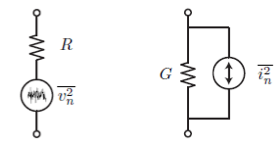
\includegraphics[scale=0.6]{pictures/widerstandrauschen}\\
\end{minipage}
\begin{minipage}{0.6\textwidth}
	\begin{align}
		Snoise(R)&=4kTR\\
		Enoise(R)&=\sqrt{4kTR}\\
		\overline{\nu^2_{n}}&=4kTRB\\
		\overline{i^2_{n}}&=4kTGB\\
		\nu_{rms} &= \sqrt{\overline{\nu^2_{n}}} = \sqrt{4kTRB}
	\end{align}
	\begin{tabular}{ll}
		B:&Bandbreite\\
		T:&Temperatur in Kelvin(293K)\\
		k:&$1.38 \cdot 10^{-23}JK^{-1}$\\
		Snoise(R):&Spektrale Dichte des Widerstandsrauschens\\
		Enoise(R):&Spannungsdichte
	\end{tabular}
\end{minipage}

\subsubsection{Widerstände in Serie}
\begin{minipage}{0.4\textwidth}
	\begin{center}
		\begin{circuitikz}[european, scale=2]
	\draw (0,0) to [R=$R1$, *-] (1,0) to [R=$R2$, -*] (2,0);
\end{circuitikz}
	\end{center}
\end{minipage}
\begin{minipage}{0.6\textwidth}
	\begin{align}
		\overline{\nu^2_{n}}&=4kT(R1+R2)B=\overline{\nu^2_{n1}}+\overline{\nu^2_{n2}}\\
		\overline{i^2_{n}}&=4kT(G1+G2)B=\overline{i^2_{n1}}+\overline{i^2_{n2}}
	\end{align}
\end{minipage}

\subsubsection{Spannungsteiler}
\begin{minipage}{0.4\textwidth}
	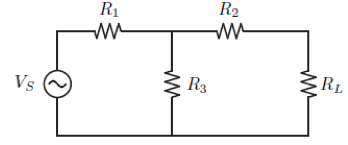
\includegraphics[scale=0.6]{pictures/seriewiderstand1}\\
	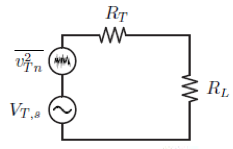
\includegraphics[scale=0.6]{pictures/seriewiderstand2}
\end{minipage}
\begin{minipage}{0.6\textwidth}
	Quellenumwandlung machen und dann Rauschen über Ersatzwiderstand ($R_T$) bestimmen.
	\begin{align}
		V_{T,s}&=V_{s}\frac{R_{3}}{R_{1}+R_{3}}\\
		\overline{\nu^2_{Tn}}&=4kTR_{T}B=4kT(R_{2}+R_{1}\parallel R_{3})B
	\end{align}
\end{minipage}

\subsection{Rauschen von RC-Netzwerken}
\begin{itemize}
  \item Kapazitäten (und Induktivitäten) rauschen nicht!
  \item Kapazitäten (und Induktivitäten) ändern die Bandbreite des Systems, d.h.
  beeinflussen dadurch die Rauschspannung
\end{itemize}
\begin{minipage}{9cm}
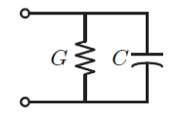
\includegraphics[scale=0.4]{pictures/rcnetzwerk}
\end{minipage}
\begin{minipage}{9cm}
\begin{gather}
Z=\frac{1}{Y}=\frac{1}{G+j\omega C}=\frac{G-j\omega C}{G^2+\omega^2C^2}\\
\overline{\nu^2_{n}}=\frac{4kT}{2\pi}\int^{\infty}_{0}\frac{G}{G^2+\omega^2C^2}d\omega=\frac{kT}{C}
\end{gather}
\end{minipage}

\subsection{Rausch-Bandbreite}
\begin{minipage}{9cm}
\begin{itemize}
  \item Nicht 3dB-Bandbreite sondern das gesamte integrierte Rauschen wird
  berechnet
  \item $e_{on}$Rauschspannung am Ausgang der Schaltung
  \item $e_{in}$Rauschspannung am Eingang der Schaltung
  \item für höhere Filterodnung\\
  \begin{tabular}{|l|l|}
  \hline
  Filter order&ENB\\\hline
  1&$1.57*f_{c}$\\\hline
  2&$1.11*f_{c}$\\\hline
  3&$1.05*f_{c}$\\\hline
  4&$1.025*f_{c}$\\\hline
  \end{tabular}\\
  ENB: Effective Noise Bandwidth
\end{itemize}

\end{minipage}
\begin{minipage}{9cm}
\begin{gather}
e_{on}=\sqrt{\int^{\infty}_{0}|A_{n(f)}|^2e^2_{in}df}\\
\text{für System 1. Ordnung}\notag\\
e_{on}=e_{in}*\sqrt{\int^{\infty}_{0}\frac{1}{1+(2\pi
fRC)^2}df}=\notag\\=e_{in}*\sqrt{\frac{1}{2\pi
RC}|^{\infty}_0\tan^{-1}2\pi fRC}=\notag\\=e_{in}\sqrt{\frac{1}{2\pi
RC}\frac{\pi}{2}}
\end{gather}
\end{minipage}

\subsection{Noise von Opamps}
\begin{minipage}{9cm}
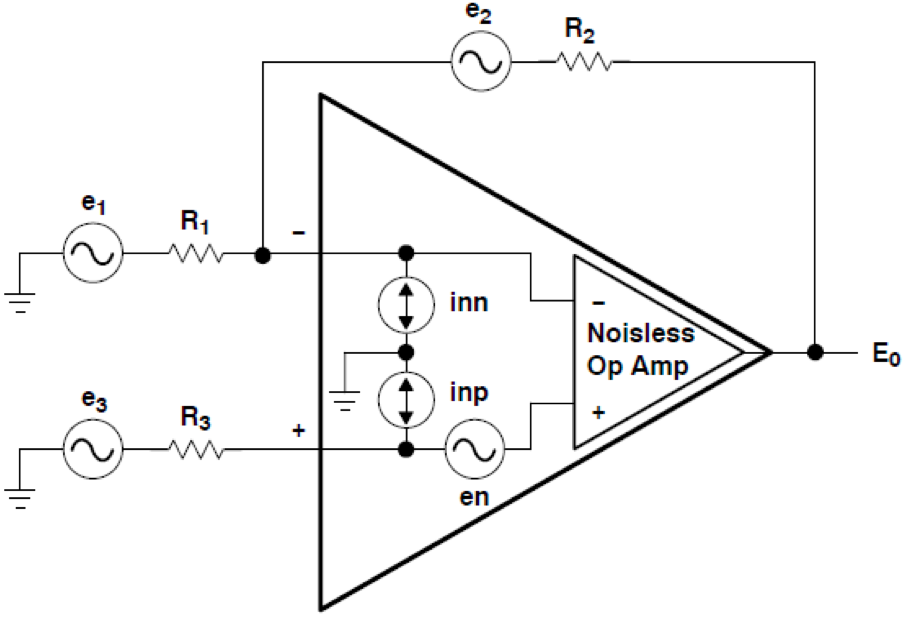
\includegraphics[scale=0.4]{pictures/oampnoise}
\end{minipage}\\
\begin{minipage}{18cm}
\textbf{Gesamtfomel (Opamp und Widerstände)}\\
\begin{gather}
E_{Trms}=\notag\\\sqrt{\int
\{4kTR_{2}(\frac{R_{1}+R_{2}}{R_{1}})+4kTR_{3}(\frac{R_{1}+R_{2}}{R_{1}})^2+((Inn)R_{2})^2+((Inn)R_{3}(\frac{R_{1}+R_{2}}{R_{1}}))^2+(e_{n}(\frac{R_{1}+R_{2}}{R_{1}}))^2\}df}
\end{gather}
\end{minipage}


Vereinfacht für CMOS-Opamps:
\begin{itemize}
  \item R3=0
  \item Gain A = $\frac{R1+R2}{R1}$
  \item $e_{w}$:Noise/root(Hz) (Aus Datenblatt)
  \item $f_{enc}$: noise corner frequenzcy (aus Datenblatt)
  \item ENB: Effective Noise Bandwidth
\end{itemize}
\begin{gather}
E_{Trms}=\sqrt{ENB4kTR_{2}A+e_{w}^2A^2(f_{enc}\ln{\frac{f_{H}}{f_{L}}}+ENB)}
\end{gather}

Ist die Bandbreite $>>f_{enc}$ ( mind. 10x grösser) kann 1/f-Noise
vernachlässigt werden
\begin{itemize}
  \item Gain A=$\frac{R1+R2}{R1}$
  \item $e_{w}$: Noise/root(Hz)(Aus Datenblatt)
  \item ENB: Effective Noise Bandwidth ($1.51*GBW/A$)
\end{itemize}
\begin{gather}
V_{noise}=\sqrt{4kT*R_{2}*A*ENB+e_{w}^2*A^2*ENB}
\end{gather}
